\section{半监督分类}
\label{sec:classification-semisupervised}

前面介绍的分类器依靠带标签的样本选择决策边界，但能够收集到的输入往往多于能够完成标注的样本。例如，积累一批待分类文档相对容易，逐篇判断主题却需要人工阅读。如果只使用已经标注的少量文档，其余文档所反映的词语共现和主题聚集结构就没有参与学习。\term{半监督分类}（semi-supervised classification）试图利用这部分信息：由真实标签确定类别含义，再借助未标注输入约束预测规则。

本节把全部$n$个样本的索引分成不相交的有标签集合$L$与无标签集合$U$，满足$L\cup U=\{1,\dots,n\}$。每个输入为$\bm{x}_i\in\mathbb{R}^{d}$，只有$i\in L$时可以在训练中使用真实标签$y_i$；除二分类的专门约定外，类别取值为$\{1,\dots,C\}$。这里的“无标签”描述算法可用的信息，不表示样本在真实任务中没有类别。标签稀缺是学习条件，树、概率模型和间隔模型则描述怎样表示或学习分类规则，因而半监督方法可以与前面几节的模型组合使用。

仅仅知道输入分布，还不能唯一确定标签如何分配。同样的两团文档，既可能对应两个主题，也可能只是写作风格不同而主题相同。因此，未标注数据能否帮助分类，取决于输入结构与类别之间是否存在可利用的联系；即使两类样本来自同一输入分布，也不能据此保证半监督训练有益。分布不匹配、标签采样偏差以及未知类别混入，还会进一步削弱这种联系。Cozman与Cohen对生成式分类器的分析给出了直接的负面结果：当建模假设与真实生成分布不一致时，加入未标注数据可能增大渐近偏差和分类错误\scite{cozman2002unlabeled}这一结论针对其分析的生成式模型，并不表示任意半监督方法都会因未标注数据而退化。

三种代表方法从不同信息入手回答这一问题。Self-Training相信经过筛选的模型预测可以补充监督；Label Propagation要求图上相邻样本的标签倾向于相似；TSVM则借助未标注样本寻找穿过低密度区域的分界面。这些条件并不互斥，也不是由弱到强的严格等级。接下来分别考察它们怎样使用无标签输入、怎样求解，以及求解成功为什么仍不等于分类一定改善。

\subsection{Self-Training}
\label{sec:classification-self-training}

已经有一个可用分类器时，最直接的办法是让它从未标注样本中挑选自己较有把握的预测，作为下一轮训练的补充。\term{自训练}（self-training）就是这样一种外层策略：基分类器负责预测，外层循环负责筛选预测并扩充训练集。用机器自身的输出代替部分教师信号的思想，在Scudder于1965年研究的自适应模式识别方法中已经出现；现代自训练的筛选、加权和重训方式则可以有许多不同实现\scite{scudder1965selftraining}

\subsubsection{模型结构}
\label{sec:classification-self-training-structure}

自训练不要求一种新的决策边界形式。基分类器仍可采用Logistic回归、SVM、决策树或随机森林；新增的部分是怎样管理暂时没有真实标签的样本。为了不混淆真实监督与模型生成的监督，保持原始$L$和$U$不变，用$A^{(t)}\subseteq U$记录第$t$轮已经采纳伪标签的样本索引，用$R^{(t)}=U\setminus A^{(t)}$记录剩余候选池。初始时$A^{(0)}=\varnothing$，模型只在$L$上训练。

假设基分类器以参数$\bm{\theta}$给出类别概率估计$p_{\bm{\theta}}(c\mid\bm{x})$。本节讨论一种阈值筛选方式，把最大类别概率作为\term{置信度}（confidence），即模型对自己当前分类结果的确定程度。对$j\in R^{(t)}$，计算
\begin{equation}
  \label{eq:classification-self-training-selection}
  \begin{aligned}
    \widehat y_j^{(t)}
      &=\argmax_{1\leq c\leq C}
        p_{\bm{\theta}^{(t)}}(c\mid\bm{x}_j),\\
    q_j^{(t)}
      &=\max_{1\leq c\leq C}
        p_{\bm{\theta}^{(t)}}(c\mid\bm{x}_j),\\
    B^{(t)}
      &=\{j\in R^{(t)}:q_j^{(t)}\geq\tau\}.
  \end{aligned}
\end{equation}
其中$\tau$是预先选择的阈值，通常取$1/C<\tau<1$；遇到并列最大值时，本节统一取编号最小的类别。被采纳的预测$\widetilde y_j=\widehat y_j^{(t)}$称为\term{伪标签}（pseudo-label）：它是模型提出的临时训练目标，并没有经过真实标注确认。本节的基本版本在采纳后固定该标签；允许重估或撤销伪标签的版本需要另外规定更新规则。

这里的概率输出是筛选接口，不是所有分类器天然具有的能力。SVM的决策分数表示带符号的间隔，不能直接当成概率与$\tau$比较；若要采用概率阈值，应使用独立标注数据拟合并检验相应的概率映射。即便分类器直接输出概率，也需要检查高置信度样本实际有多可靠。在一个教学例子中，二分类预测$(0.96,0.04)$会通过$\tau=0.9$的筛选，而$(0.55,0.45)$不会；这一筛选只说明前者符合模型的接受条件，并没有证明前者的真实类别就是1。

\subsubsection{参数学习}
\label{sec:classification-self-training-learning}

每轮采纳伪标签后，基分类器需要重新拟合。以可加权的损失$\ell$为例，当前训练目标可以写成
\begin{equation}
  \label{eq:classification-self-training-objective}
  \begin{aligned}
    \mathcal{J}_t(\bm{\theta})
      ={}&\frac{1}{|L|}\sum_{i\in L}
        \ell\bigl(f_{\bm{\theta}}(\bm{x}_i),y_i\bigr)\\
      &+\frac{\eta}{\max\{1,|A^{(t)}|\}}
        \sum_{j\in A^{(t)}}
        \ell\bigl(f_{\bm{\theta}}(\bm{x}_j),\widetilde y_j\bigr)\\
      &+\beta\Omega(\bm{\theta}).
  \end{aligned}
\end{equation}
这里$L$非空，$\eta\geq0$控制伪标签项的相对权重，$\beta\Omega$沿用基分类器的正则化方式。空伪标签集的求和取零。分别归一化两类样本，是为了避免仅因伪标签数量增加就让它们压过真实标签；若采用统一样本权重，其相对影响会随集合大小改变。对于树等不直接求解这个目标的分类器，可以使用对应的带权拟合接口，自训练的集合更新逻辑不变。

算法\ref{alg:classification-self-training}给出固定阈值、固定已采纳伪标签的版本。$\operatorname{Fit}(A)$表示用真实标签集与索引为$A$的伪标签集完成一次基分类器训练，并返回参数；式~\eqref{eq:classification-self-training-objective}~是这种训练的一种具体实现。算法中省略集合的迭代上标，始终让当前参数对应当前已采纳的训练集。

\begin{algorithm}[带最终重训的自训练]
  \label{alg:classification-self-training}
  \begin{algorithmic}[1]
    \Require 有标签索引$L$、无标签索引$U$及其输入
    \Require 阈值$\tau$、最大扩充轮数$T\geq0$
    \Ensure 分类器$f_{\bm{\theta}}$、已采纳索引$A$和剩余索引$R$
    \State $A\gets\varnothing$，$R\gets U$
    \State $\bm{\theta}\gets\operatorname{Fit}(A)$
    \For{$t=1,\dots,T$}
      \If{$R=\varnothing$}
        \State \textbf{break}
      \EndIf
      \State 用当前模型计算$R$中的$\widehat y_j$与$q_j$
      \State $B\gets\{j\in R:q_j\geq\tau\}$
      \If{$B=\varnothing$}
        \State \textbf{break}
      \EndIf
      \State 保存$\widetilde y_j\gets\widehat y_j$，$j\in B$
      \State $A\gets A\cup B$，$R\gets R\setminus B$
      \State $\bm{\theta}\gets\operatorname{Fit}(A)$
    \EndFor
    \State \Return $f_{\bm{\theta}},A,R$
  \end{algorithmic}
\end{algorithm}

把重训放在集合扩充之后有一个直接作用：无论这一轮恰好用完最大轮数，还是把剩余池清空，返回的模型都已经使用了本轮加入的伪标签。若把训练放在循环开头、随后只添加样本就退出，最后一批伪标签实际上不会影响返回模型。预测前检查空池也很必要，空输入未必被基分类器的批量预测接口接受。当$U$为空或$T=0$时，算法自然返回纯监督模型。

图\ref{fig:classification-self-training}把算法中的集合变化与模型反馈放在同一条流程中。应注意返回预测步骤的箭头：它传回的是用新增伪标签重训后的模型，而不是一批经过人工确认的标签。真实标签始终固定在$L$中；未通过筛选的样本仍留在$R$，已采纳的样本进入$A$，也不会因此成为真实标注样本。

\begin{figure*}[htbp]
  \centering
  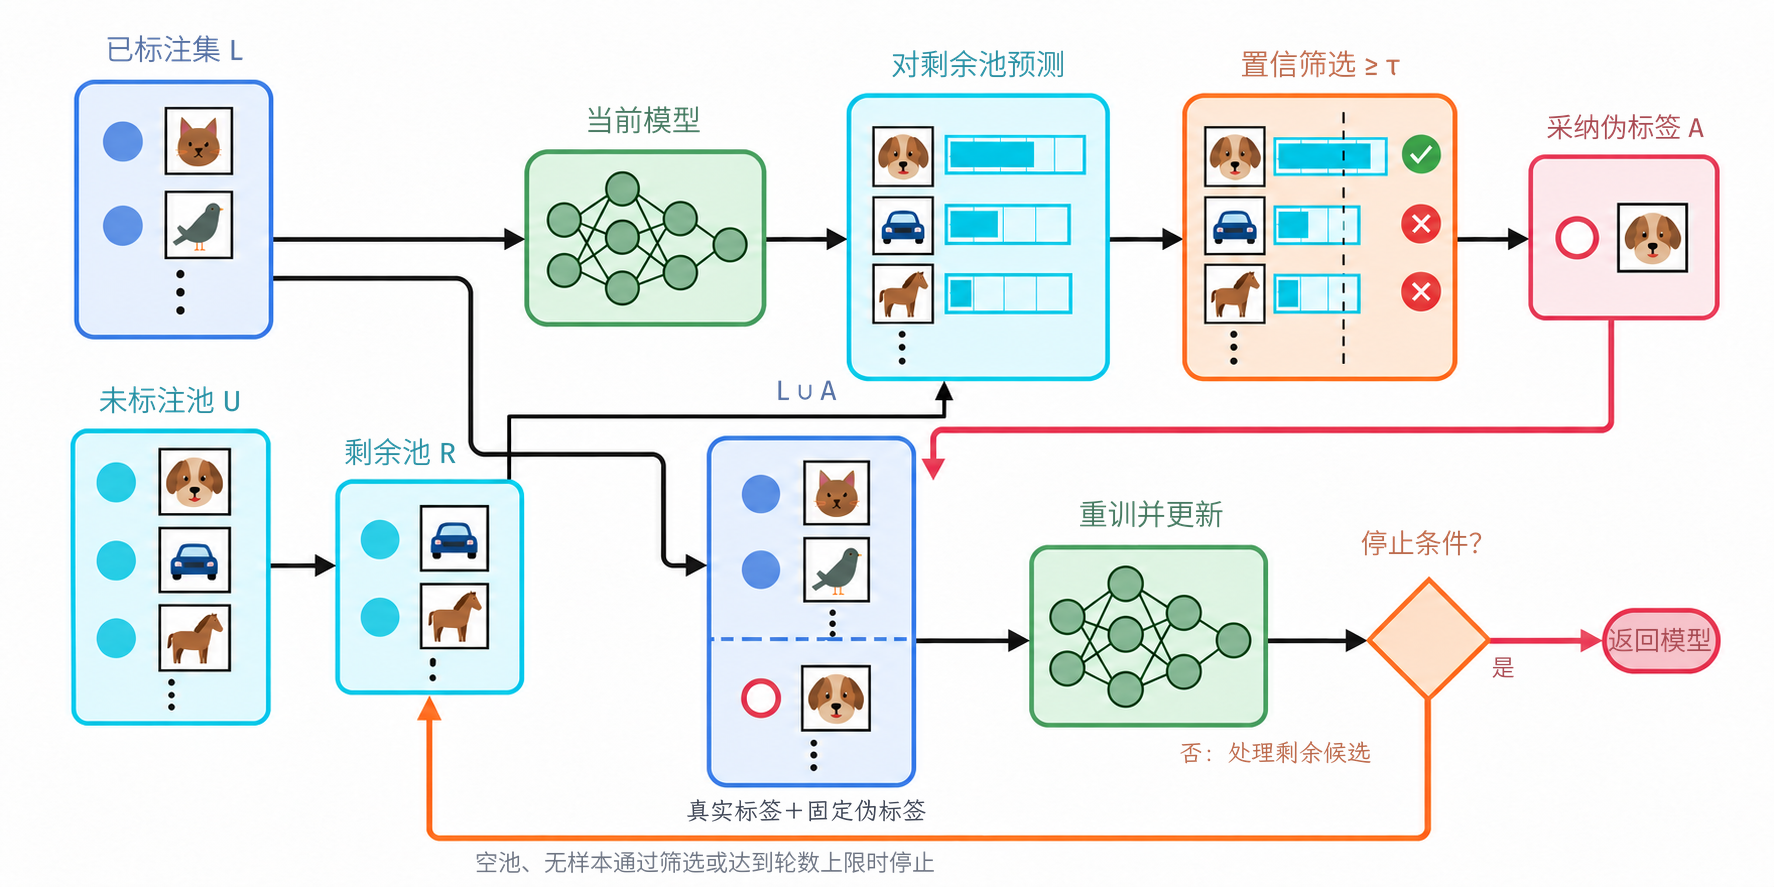
\includegraphics[width=\linewidth]{figures/03-models/01-classic-models/generated/classification-self-training/figure.png}
  \caption{固定阈值、固定已采纳伪标签的自训练流程，对应算法~\ref{alg:classification-self-training}。真实标签保持不变，已采纳的伪标签始终是模型预测。每次采纳后先重训，再用更新后的模型处理剩余候选；空池、无样本通过筛选或达到轮数上限时停止。这个模型反馈回路也可能产生确认偏差：错误预测被当作后续监督，使模型进一步强化原有误判。}
  \label{fig:classification-self-training}
\end{figure*}

阈值并非唯一的筛选手段。每轮可以只采纳通过阈值的前若干个样本，以控制一次错误扩充的影响；也可以按类别限制数量，避免某个易预测类别占据全部新增监督。这些策略改变的是$B^{(t)}$的构造，不改变先保存标签、再扩充集合、随后重训的顺序。类别配额应参考真实任务中的类别比例，不能为了数量整齐就把不平衡任务强行改成均衡任务。

\subsubsection{理论分析}
\label{sec:classification-self-training-analysis}

\paragraph{收敛性分析}
这个基本版本何时停止，可以直接从集合变化判断。每次成功扩充至少从$R$移走一个样本，且样本不会移回，因此成功扩充最多发生$\min\{T,|U|\}$次；若没有样本通过筛选，循环会更早结束。只要每次基分类器训练能够返回，外层循环就会有限终止。这不是对统计最优性的证明，也不代表一列参数收敛到某个固定目标的全局极小值，因为训练集及其监督信号一直在变化。

自训练与\term{熵最小化}（entropy minimization）有共同的倾向：都可能让未标注样本上的预测变得更确定。熵最小化直接惩罚模型预测分布的条件熵，推动概率集中到少数类别。Grandvalet与Bengio讨论了这一准则及其与自训练的联系，但这种联系依赖具体的概率模型和优化设定，不能把所有硬伪标签流程都视为同一个优化问题\scite{grandvalet2004entropy}

对一个未标注输入$\bm{x}$，Shannon熵与硬伪标签交叉熵分别涉及
\begin{equation}
  \label{eq:classification-pseudolabel-entropy}
  \begin{aligned}
    H_{\bm{\theta}}(\bm{x})
      &=-\sum_{c=1}^{C}p_{\bm{\theta}}(c\mid\bm{x})
        \log p_{\bm{\theta}}(c\mid\bm{x}),\\
    \min_{\widetilde y\in\{1,\dots,C\}}
      \{-\log p_{\bm{\theta}}(\widetilde y\mid\bm{x})\}
      &=-\log\max_c p_{\bm{\theta}}(c\mid\bm{x}).
  \end{aligned}
\end{equation}
前者对所有类别求加权和，后者只取概率最大的一个类别，两者数值和梯度一般不同。例如，预测为$(0.8,0.2)$时，以自然对数计算的熵约为$0.500$，最小硬标签交叉熵约为$0.223$。实际自训练还会筛选样本并冻结历史伪标签，因此下一轮甚至不一定仍以当前最大概率类别为目标。

\paragraph{泛化分析}
在平滑性与模型容量约束合适时，提升同一聚集区域内的预测确定性，可能促使决策边界远离该区域；但仅在单个输入上降低熵，并不自动约束附近输入的分类。更关键的是，熵只衡量确定程度，不衡量答案是否正确。若初始分类器错误地把一批同主题文档判成另一类，采纳这些预测后再训练，模型可能对原错误更加确信。这种把自身误判重新当作证据的现象称为\term{确认偏差}（confirmation bias）。Arazo等在深度图像分类实验中观察到，朴素伪标签训练会拟合错误伪标签，并比较了缓解这一现象的正则化方法\scite{arazo2020confirmation}这项证据支持错误可能被反馈回路强化，不构成所有自训练流程必然恶化的普遍定理。

伪标签错误怎样影响真实风险，可以在固定一轮模型后直接推导。令$h$为这一轮产生伪标签的分类器，$\bm{X}_\tau\subseteq\mathbb{R}^{d}$为通过其置信度阈值的输入区域。对目标分布$\mathcal{P}$，用$R_{\mathcal{P}}(f)=\mathbb{P}_{\mathcal{P}}(f(\bm{x})\ne y)$表示任意候选分类器$f$的新样本风险。设$\pi=\mathbb{P}_{\mathcal{P}}(\bm{x}\in\bm{X}_\tau)>0$，在筛选区域内分别考察伪标签自身的错误率，以及$f$与伪标签不一致的概率：
\begin{equation}
  \label{eq:classification-self-training-conditional-risks}
  \begin{aligned}
    e_\tau
      &=\mathbb{P}_{\mathcal{P}}
        \bigl(h(\bm{x})\ne y\mid\bm{x}\in\bm{X}_\tau\bigr),\\
    \widetilde R_\tau(f)
      &=\mathbb{P}_{\mathcal{P}}
        \bigl(f(\bm{x})\ne h(\bm{x})\mid\bm{x}\in\bm{X}_\tau\bigr).
  \end{aligned}
\end{equation}
若$f$预测错误，它要么与$h$不一致，要么沿用了$h$的错误，因此
\begin{equation}
  \label{eq:classification-self-training-error-events}
  \{f(\bm{x})\ne y\}
    \subseteq
    \{f(\bm{x})\ne h(\bm{x})\}
    \cup\{h(\bm{x})\ne y\},
\end{equation}
在$\bm{X}_\tau$内应用并集界，再把区域内外的风险相加，得到
\begin{equation}
  \label{eq:classification-self-training-risk}
  \begin{aligned}
    R_{\mathcal{P}}(f)
      \leq{}&\pi\bigl(\widetilde R_\tau(f)+e_\tau\bigr)\\
      &+\mathbb{P}_{\mathcal{P}}
        \bigl(f(\bm{x})\ne y,\ \bm{x}\notin\bm{X}_\tau\bigr).
  \end{aligned}
\end{equation}
因此，即使$f$完全拟合了该区域的伪标签，也不能据此消除$e_\tau$，更没有控制区域外的错误。这个界描述固定一轮模型及其筛选区域的总体风险关系，不是多轮自训练的风险递减定理；$\widetilde R_\tau(f)$也不是有限伪标签集上的训练误差。采纳事件依赖模型，历史伪标签又由不同轮次产生，不能把$|L|+|A|$直接当成独立真实标签的样本数来套用监督泛化界。

较高阈值能够减少采纳数量，却不能消除系统性高置信度错误。控制伪标签权重与单轮规模、检验不同类别的接受率，以及用保留的真实标签验证集比较扩充前后的性能，分别约束影响强度、类别偏置与实际效果。验证样本不能同时作为被模型反复吸收的伪标签训练样本，否则对自训练收益的估计会失去独立性。若未标注池混入未知类别，或标注数据只覆盖少数容易区域，还需要检查这些不匹配，而不能只调低阈值以追求更多伪标签。

\subsubsection{小结}
\label{sec:classification-self-training-summary}

自训练把已有分类器的部分预测转化为新增监督，适合在保留原有训练和预测接口的情况下探索无标签数据的价值。它的额外成本包括对剩余池反复预测，以及在不断扩大的训练集上重新拟合；基分类器训练昂贵时，这些成本并不小。最终模型仍按原分类器的方式预测新样本，无须保留一个独立的传播图。

是否采用自训练，主要取决于初始预测能否筛出足够可靠且有代表性的样本。标签极少时，恰恰可能无法满足这一条件，所以它不是所有冷启动任务的默认答案；反过来，具备持续验证和错误处理机制时，也没有理由把它限定为只能短期使用。人工复核可以改善部分伪标签的质量，但是否需要、复核哪些样本，应由误判代价与可用预算决定，不能把这一环节当作普遍充分的安全保证。

\subsection{Label Propagation}
\label{sec:classification-label-propagation}

自训练通过基分类器决定哪些预测值得采纳；如果可信的信息主要来自样本之间的邻近关系，也可以直接在这些关系上传递标签。\term{标签传播}（label propagation）把样本表示为图的节点，让已有标签沿相似边影响尚无标签的节点。Zhu与Ghahramani在2002年的技术报告中给出了保持已知标签不变的传播方法\scite{zhu2002labelpropagation}与只在已标注样本中寻找近邻相比，未标注点也参与形成传播路径，使标签能够沿弯曲的高密度区域传递；每轮恢复已知标签，则让它们持续提供监督，不会因反复平均而失去原有的类别信息。

本节采用与调和函数解释一致的随机游走记号，明确区分这种硬边界传播与后面介绍的软约束版本。

\subsubsection{模型结构}
\label{sec:classification-label-propagation-structure}

图模型把“哪些输入相似”转化成可计算的边权。令$\mathcal{G}=(V,E,\bm{W})$，其中$V=L\cup U$，$\bm{W}\in\mathbb{R}^{n\times n}$为非负对称权重矩阵，$\bm{W}_{i,j}=\bm{W}_{j,i}\geq0$，且取$\bm{W}_{i,i}=0$。例如，可以先选出近邻边，再在相连节点上使用RBF相似度
\begin{equation}
  \label{eq:classification-label-propagation-weights}
  \bm{W}_{i,j}=
  \begin{cases}
    \exp\bigl(-\gamma\lVert\bm{x}_i-\bm{x}_j\rVert_2^2\bigr),
      & \{i,j\}\in E,\\
    0, & \text{其他情形},
  \end{cases}
\end{equation}
其中$\gamma>0$控制相似度衰减。用$k$近邻关系构图时，单向近邻关系需要经过并集或互近邻等明确规则转成无向边，才能满足对称性。完全图保留所有样本对，稀疏图只保留选中的关系；两者不仅存储成本不同，也可能给出不同的分类结果。

每个节点的加权度记为$\delta_i=\sum_j\bm{W}_{i,j}$，度矩阵满足$\bm{D}_{i,i}=\delta_i$。在所有参与传播的节点度数为正时，定义
\begin{equation}
  \label{eq:classification-label-propagation-transition}
  \bm{P}=\bm{D}^{-1}\bm{W},
  \qquad
  \bm{P}_{i,j}=\frac{\bm{W}_{i,j}}{\delta_i}.
\end{equation}
矩阵$\bm{P}$每行的和为1，表示从一个节点沿边随机走向邻居的转移概率。传播时用这一行权重对邻居的标签信息求平均；权重大，邻居的影响也大。

为了同时处理$C$个类别，令$\bm{F}\in\mathbb{R}^{n\times C}$保存节点得分，$\bm{f}_i=(\bm{F}_{i,1},\dots,\bm{F}_{i,C})^\top$为节点$i$的得分向量。构造同形状的$\bm{Y}$：若$i\in L$，则$\bm{Y}_{i,c}=\mathbb{1}\{y_i=c\}$；若$i\in U$，则整行置零。有标签节点在每轮更新后都恢复到这份独热编码，这种固定边界的操作称为\term{硬钳制}（hard clamping），也就是不允许传播改变已经给定的标签。

构图时必须检查标签信息能否到达每个待预测节点。零度无标签节点没有邻居，无法定义式~\eqref{eq:classification-label-propagation-transition}~中的转移概率；一个连通分量若完全没有标签，即使每个节点度数都大于零，也无法确定任何类别。可以补充真实标签、依据可靠关系重新构图，或对这些节点明确拒绝预测。孤立的有标签节点保留原标签即可，不必参与传播。仅增加一个微小度数或自环，只解决部分数值形式问题，并没有给缺少监督的分量提供类别信息。

\subsubsection{参数学习}
\label{sec:classification-label-propagation-learning}

标签传播没有固定维数的分类器参数要拟合，但需要求出全部无标签节点的得分。下面假设零度节点已经处理，每个含无标签节点的连通分量至少含一个有标签节点。把$\bm{F}$按$L$与$U$分成行块$\bm{F}_L=\bm{F}_{L,:}$、$\bm{F}_U=\bm{F}_{U,:}$，并对$\bm{P}$作对应分块。硬钳制意味着$\bm{F}_L^{(t)}=\bm{Y}_L$始终不变，因而只需迭代
\begin{equation}
  \label{eq:classification-label-propagation-iteration}
  \bm{F}_U^{(t+1)}
    =\bm{P}_{U,U}\bm{F}_U^{(t)}
     +\bm{P}_{U,L}\bm{Y}_L.
\end{equation}
右侧第一项传递尚无标签节点之间的当前信息，第二项持续注入真实标签。通常取$\bm{F}_U^{(0)}=\bm{0}$。这个硬钳制方案不需要再引入传播系数$\alpha$，也不在有标签节点上附加一个有限权重的软拟合项。

若迭代达到固定点，移项便得到线性系统与形式上的闭式解
\begin{equation}
  \label{eq:classification-label-propagation-solution}
  \begin{aligned}
    (\bm{I}-\bm{P}_{U,U})\bm{F}_U^\ast
      &=\bm{P}_{U,L}\bm{Y}_L,\\
    \bm{F}_U^\ast
      &=(\bm{I}-\bm{P}_{U,U})^{-1}
        \bm{P}_{U,L}\bm{Y}_L.
  \end{aligned}
\end{equation}
这里$\bm{I}$为$|U|\times|U|$单位矩阵。下一小节将证明，在上述图条件下逆矩阵存在，且任意初始化的迭代都收敛到同一个解。计算时通常直接求解线性系统，避免显式构造逆矩阵。Zhu、Ghahramani与Lafferty给出了这一解的调和函数、图能量和随机游走解释\scite{zhu2003}

图\ref{fig:classification-label-propagation}给出一个可逐项核算的教学构造，并非实测数据。五个节点依次相连，每条无向边的权重为1；端点1固定属于类1，端点5固定属于类2，节点2、3、4没有标签。令$p_i=\bm{F}_{i,1}^\ast$，由于每个内点恰有两个等权邻居，式~\eqref{eq:classification-label-propagation-iteration}~在固定点处变为
\begin{equation}
  \label{eq:classification-label-propagation-path}
  \begin{aligned}
    p_i&=\frac{p_{i-1}+p_{i+1}}{2},
      &&i=2,3,4,\\
    p_1&=1,\qquad p_5=0.
  \end{aligned}
\end{equation}
内点方程等价于$p_{i+1}-p_i=p_i-p_{i-1}$，所以相邻节点的得分差必须相等。两端总共下降1，分到四条边上，每步下降$1/4$，得到
\[
  (p_1,p_2,p_3,p_4,p_5)
    =(1,0.75,0.5,0.25,0).
\]
类2的得分满足相反的端点条件，故$\bm{f}_i^\ast=(p_i,1-p_i)^\top$。节点2偏向类1，节点4偏向类2；节点3的两类得分相同，按本节“并列时取最小类别编号”的约定判为类1。这个离散判定只是处理并列的规则，不能被解释为节点3存在支持类1的额外证据。

\begin{figure}[htbp]
  \centering
  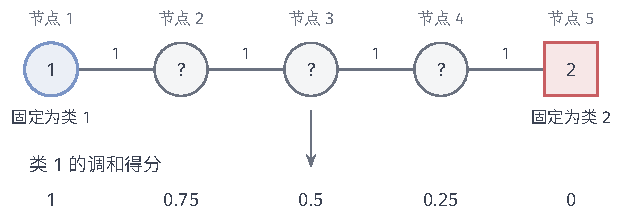
\includegraphics[width=\linewidth]{figures/03-models/01-classic-models/tikz/classification-label-propagation/figure.pdf}
  \caption{五节点等权无向路径上的硬钳制标签传播。每条边权为1，左端圆形节点固定为类1，右端方形节点固定为类2，问号表示未知标签。下方列出精确调和解的类1得分，类2得分为其补数；内点得分等于两侧邻居的平均。中间节点两类并列，按最小类别编号规则判为类1。这是教学构造，不是实测结果。}
  \label{fig:classification-label-propagation}
\end{figure}

迭代实现还需要把停止条件与返回值对应起来。算法\ref{alg:classification-label-propagation}使用相邻两轮之差作为数值停止判据，其中$\lVert\cdot\rVert_{\mathrm{F}}$为Frobenius范数，$\varepsilon>0$为容限，$T\geq1$为最大迭代次数。若达到上限时仍未满足容限，返回的状态必须保留这一信息，不能把“运行结束”报告为“已经收敛”。

\begin{algorithm}[硬钳制标签传播]
  \label{alg:classification-label-propagation}
  \begin{algorithmic}[1]
    \Require 权重$\bm{W}$、索引$L,U$、标签矩阵$\bm{Y}$
    \Require 容限$\varepsilon>0$、最大迭代次数$T\geq1$
    \Ensure 得分$\bm{F}$、预测$\widehat{\bm{y}}_U$及停止状态
    \If{$U=\varnothing$}
      \State \Return $\bm{Y}$、空预测、已完成
    \EndIf
    \State 检查$\bm{W}$非负、对称，参与传播的节点度数为正
    \State 检查每个含$U$节点的连通分量至少有一个$L$节点
    \If{任何检查失败}
      \State \Return 拒绝结果，要求补标签或修正传播图
    \EndIf
    \State 构造$\bm{P}=\bm{D}^{-1}\bm{W}$
    \State $\bm{F}_L\gets\bm{Y}_L$，$\bm{F}_U\gets\bm{0}$
    \State $\mathrm{converged}\gets\mathrm{false}$
    \For{$t=1,\dots,T$}
      \State $\bm{G}\gets\bm{P}_{U,U}\bm{F}_U+\bm{P}_{U,L}\bm{Y}_L$
      \State $\Delta\gets\lVert\bm{G}-\bm{F}_U\rVert_{\mathrm{F}}$
      \State $\bm{F}_U\gets\bm{G}$
      \If{$\Delta\leq\varepsilon(1+\lVert\bm{F}_U\rVert_{\mathrm{F}})$}
        \State $\mathrm{converged}\gets\mathrm{true}$
        \State \textbf{break}
      \EndIf
    \EndFor
    \State $\widehat y_j\gets\argmax_c\bm{F}_{j,c}$，$j\in U$；并列取最小$c$
    \State \Return $\bm{F},\widehat{\bm{y}}_U,\mathrm{converged}$
  \end{algorithmic}
\end{algorithm}

算法先把$\bm{G}$保存成最新的$\bm{F}_U$，再判断是否退出，因此即使本轮达到容限，也会返回新得分而不是上一轮的值。相邻迭代差小是一种可操作的停止指标，不直接给出距离精确解的统一误差界；当传播很慢时，还需结合线性系统残差与条件数判断数值精度。最终类别由得分比较决定，接近平局的节点尤其需要保留得分与未收敛状态。

\subsubsection{理论分析}
\label{sec:classification-label-propagation-analysis}

\paragraph{收敛性分析}
硬钳制传播能够收敛，关键不是“每个节点都直接连着标签”，而是未标注节点经过若干步能够到达有标签节点。$\bm{P}_{U,U}$每一行的和至多为1，其中某些行可以恰好等于1，因为对应节点暂时只有无标签邻居。要证明收缩，需要考察多步传播后仍然留在$U$中的总权重。

\begin{theorem}[硬钳制传播的唯一解]
  \label{thm:classification-label-propagation-convergence}
  设图有限、边权非负且对称，所有参与传播的节点度数为正，$U$非空，且每个含无标签节点的连通分量至少含一个有标签节点。则$\rho(\bm{P}_{U,U})<1$，其中$\rho$表示谱半径。式~\eqref{eq:classification-label-propagation-iteration}~从任意初始得分出发，都收敛到式~\eqref{eq:classification-label-propagation-solution}~中的唯一固定点。
\end{theorem}

\begin{proof}
  从每个$j\in U$出发，选择一条到达$L$的正权路径，并在首次到达$L$时停止。有限图中这些路径长度有一个共同上界$m$，沿各路径行走的概率均为正，其最小值记为$\epsilon>0$。于是，无论从哪个无标签节点出发，在$m$步以内命中$L$的概率都至少为$\epsilon$。这说明
  \[
    \lVert\bm{P}_{U,U}^{m}\rVert_\infty\leq1-\epsilon,
    \qquad
    \rho(\bm{P}_{U,U})^m\leq1-\epsilon<1.
  \]
  因而$\bm{P}_{U,U}^t$趋于零，Neumann级数收敛，且
  \[
    (\bm{I}-\bm{P}_{U,U})^{-1}
      =\sum_{t=0}^{\infty}\bm{P}_{U,U}^{t}.
  \]
  迭代展开为
  \[
    \bm{F}_U^{(t)}
      =\bm{P}_{U,U}^{t}\bm{F}_U^{(0)}
       +\sum_{s=0}^{t-1}
         \bm{P}_{U,U}^{s}\bm{P}_{U,L}\bm{Y}_L.
  \]
  第一项消失，第二项趋于所述固定点。逆矩阵存在，也排除了其他固定点。
\end{proof}

还可以从最优化的角度解释同一个解。相邻节点的得分差越大，图上的不平滑程度越高。令$\bm{L}_{\mathrm{g}}=\bm{D}-\bm{W}$为\term{图拉普拉斯矩阵}（graph Laplacian），它把这种局部差异汇总成二次型。固定真实标签边界后，求解的\term{狄利克雷能量}（Dirichlet energy）最小化问题为
\begin{equation}
  \label{eq:classification-label-propagation-energy}
  \begin{aligned}
    \min_{\bm{F}:\,\bm{F}_L=\bm{Y}_L}\quad
    \mathcal{E}(\bm{F})
      &=\frac12\sum_{i,j=1}^{n}
        \bm{W}_{i,j}\lVert\bm{f}_i-\bm{f}_j\rVert_2^2\\
      &=\operatorname{tr}
        (\bm{F}^{\top}\bm{L}_{\mathrm{g}}\bm{F}).
  \end{aligned}
\end{equation}
第\ref{sec:clustering-spectral}节的谱聚类与第\ref{sec:dim-le}节的拉普拉斯特征映射复用图拉普拉斯和谱工具，但输出分别是离散簇分配与连续低维坐标；这里的标签传播则在已知类别语义下求类别得分。共享图结构不意味着三个任务使用相同的输出约束。

有标签节点在这里是固定边界，不是可以通过支付有限罚项而改变的变量。对未知行块求导并令其为零，得到
\begin{equation}
  \label{eq:classification-label-propagation-dirichlet}
  \begin{aligned}
    (\bm{L}_{\mathrm{g}})_{U,U}\bm{F}_U
      &=-(\bm{L}_{\mathrm{g}})_{U,L}\bm{Y}_L\\
      &=\bm{W}_{U,L}\bm{Y}_L.
  \end{aligned}
\end{equation}
因为$(\bm{L}_{\mathrm{g}})_{U,U}=\bm{D}_{U,U}-\bm{W}_{U,U}$，左乘$\bm{D}_{U,U}^{-1}$就回到式~\eqref{eq:classification-label-propagation-solution}~的线性系统。

这个驻点也是唯一最小值，而不只是一个形式上的导数解。取任意无标签节点上的非零向量$\bm{z}$，把它扩展成在$L$上为零的全图向量$\widetilde{\bm{z}}$，则
\[
  \bm{z}^{\top}(\bm{L}_{\mathrm{g}})_{U,U}\bm{z}
    =\frac12\sum_{i,j}\bm{W}_{i,j}
      (\widetilde z_i-\widetilde z_j)^2.
\]
右侧若为零，向量在每个正权连通分量上就必须为常数。每个涉及$U$的分量又含一个值为零的标签边界，因此这些常数只能全部为零，与$\bm{z}\ne\bm{0}$矛盾。故未标记主子块正定，能量对$\bm{F}_U$严格凸。这同时解释了为什么完全无标签的分量会破坏唯一性：在这种分量上，任意常值向量都不增加图能量。

得分的概率含义也需要依赖这些条件。从一个无标签节点按$\bm{P}$行走，并在首次碰到有标签节点时停止，$\bm{F}_{j,c}^\ast$等于首次命中的标签属于类$c$的概率。由于最终命中$L$的概率为1，精确解各行非负且行和为1。若从零初始化，有限轮得分只累积了相应步数内的命中概率，行和可能还小于1；一般不能把尚未收敛的得分直接当成归一化概率。即便在极限处，这也是给定图上的命中概率，不自动等于真实任务中校准的类别后验。

\paragraph{泛化分析}
优化的唯一性没有检验图是否表达了正确的类别关系。\term{平滑假设}（smoothness assumption）在这里意味着强相似边连接的节点应具有相近标签得分；若文档按写作风格聚集却按主题分类，这个假设就可能失效。跨类强边会把错误信息传到邻域，错误的标签边界还会被硬钳制持续保留。高维距离失真时，特征标准化、降维或度量学习可以改善构图的候选表示，但这些处理同样需要验证，不能由线性系统收敛来证明其合理性。

这里还要区分两种评价对象。对非空$U$，在训练之外取得真实标签后，可以计算
\begin{equation}
  \label{eq:classification-label-propagation-pool-risk}
  \widehat R_U
    =\frac{1}{|U|}\sum_{j\in U}
      \mathbb{1}\{\argmax_c\bm{F}_{j,c}^\ast\ne y_j\}.
\end{equation}
其中并列得分仍按最小类别编号处理，$y_j$只用于评价。这个误差针对已经参与构图的输入，不是对未来独立样本风险的直接估计。要讨论新样本，还必须定义归纳扩展$h_{\mathcal{G}}(\bm{x})$，即规定新输入如何连接到图、怎样由图上得分产生预测，以及是否重新求解；这时才有相应的风险$R_{\mathcal{P}}(h_{\mathcal{G}})=\mathbb{P}_{\mathcal{P}}(h_{\mathcal{G}}(\bm{x})\ne y)$。

前述定理没有对$R_{\mathcal{P}}(h_{\mathcal{G}})$给出上界：它既未规定这种扩展，也未假设新样本与图上标签之间的统计关系。若要建立随样本数变化的风险保证，还需把构图规则、标签覆盖和类别平滑性等条件与目标分布联系起来。对一个给定图求出唯一解，只解决了得分怎样确定，不能替代这些条件。

\subsubsection{小结}
\label{sec:classification-label-propagation-summary}

标签传播适合相似关系本身可信的任务，例如有可靠连接语义的节点分类，或用局部外观关系传播图像块标签。其基本输出是当前图上各节点的得分，适合面向这批输入作出预测；若任务持续接收新输入，前述归纳扩展也应纳入模型设计和评价。

计算成本取决于图的稀疏性与求解精度，而不是一个固定的节点数分界。记$\operatorname{nnz}(\bm{W})$为非零权重数，稀疏图一次传播的主要乘法成本为$O(\operatorname{nnz}(\bm{W})C)$，存储主要为$O(\operatorname{nnz}(\bm{W})+nC)$；总时间还要乘以迭代次数，并另计构图成本。完全图的存储为$O(n^2)$，直接计算所有欧氏距离通常需$O(n^2d)$。即使图很稀疏，连接标签区域的边过弱，也会使$\rho(\bm{P}_{U,U})$接近1，导致传播缓慢。

可以利用稀疏线性求解器，或在合适的相似度矩阵上使用\term{Nyström近似}（Nyström approximation），即选取少量代表列来构造低秩近似，减少矩阵运算。但近似相似度不一定保留原图的非负边权、连通关系与硬边界解；采用近似后应重新检查这些条件和求解误差。图上的唯一解、数值上的近似精度以及分类准确率，是三个需要分别评价的问题。

\subsection{TSVM}
\label{sec:classification-tsvm}

图传播直接平滑节点得分；若希望保留SVM的分类函数，则可以让无标签样本参与选择大间隔边界。\term{直推支持向量机}（transductive support vector machine, TSVM）同时选择分类器与当前未标注样本的标签，使两类样本共同约束间隔。Joachims在1999年的文本分类研究中给出了有代表性的目标与实用求解算法。其相关性反馈任务说明了这一选择的背景：用户只标注少量检索结果是否相关，其余待分类文档却已经构成一个给定的文档库。于是，这些文档不必等到训练结束后才交给分类器，而可以在训练时通过自身的位置参与确定间隔边界\scite{joachims1999transductive}

这里的\term{直推学习}（transductive learning，也称转导学习）指利用当前已给定的待预测输入，直接推断这批输入的标签；它与面向未来新输入评价预测规则的归纳设定有所区别。TSVM仍会得到一个SVM分类函数，所以从计算上也能处理新样本。区别在于哪些输入参与了训练，以及理论或实验评价针对哪批预测，而不是算法是否能够写出一个函数。

\subsubsection{模型结构}
\label{sec:classification-tsvm-structure}

本小节使用二分类标签$\{-1,+1\}$。令$g(\bm{x})=\bm{w}^{\top}\phi(\bm{x})+b$为决策分数，$\phi$为选定的特征映射；线性SVM取$\phi(\bm{x})=\bm{x}$。标准软间隔SVM只要求已标注样本尽量满足$y_i g(\bm{x}_i)\geq1$。TSVM还为每个$j\in U$引入一个待选择的离散标签$y_j^{\mathrm{u}}$，并为相应间隔约束配置松弛变量$\xi_j^{\mathrm{u}}$。其目标可写为
\begin{equation}
  \label{eq:classification-tsvm-objective}
  \begin{aligned}
    \min_{\bm{w},b,\bm{y}^{\mathrm{u}},\bm{\xi}}\quad
    \mathcal{J}
      ={}&\frac12\lVert\bm{w}\rVert_2^2
         +\lambda_{\mathrm{s}}\sum_{i\in L}\xi_i\\
       &+\lambda_{\mathrm{u}}\sum_{j\in U}\xi_j^{\mathrm{u}},
  \end{aligned}
\end{equation}
其中$\bm{y}^{\mathrm{u}}$收集无标签节点的离散标签，$\bm{\xi}$收集两类松弛变量，$\lambda_{\mathrm{s}}>0$与$\lambda_{\mathrm{u}}\geq0$分别控制有标签项和无标签项的惩罚。约束为
\begin{equation}
  \label{eq:classification-tsvm-constraints}
  \begin{aligned}
    y_i g(\bm{x}_i)&\geq1-\xi_i,
      &\xi_i&\geq0,\quad i\in L,\\
    y_j^{\mathrm{u}}g(\bm{x}_j)&\geq1-\xi_j^{\mathrm{u}},
      &\xi_j^{\mathrm{u}}&\geq0,\quad j\in U,\\
    y_j^{\mathrm{u}}&\in\{-1,+1\},
      &&j\in U,\\
    \sum_{j\in U}\frac{1+y_j^{\mathrm{u}}}{2}&=r.
  \end{aligned}
\end{equation}
最后一行固定无标签样本中的正类标签数量$r$。本节讨论$|U|\geq2$且$1\leq r\leq|U|-1$的非退化情形；$\lambda_{\mathrm{u}}=0$或$U$为空时，分类器训练回到纯监督SVM。

类别数量约束来自一个实际困难：无标签样本本身不能说明哪一侧应有多少样本。若只要求间隔大，模型可能把几乎全部未标注样本放到同一类，从而得到不符合任务的划分。\term{类别平衡约束}（class-balance constraint）把对类别组成的外部知识加入优化，它不要求两类数量相等，而是固定或限制可接受的比例。可以根据可信先验选择$r$，也可以规定$r_{\min}\leq\sum_j(1+y_j^{\mathrm{u}})/2\leq r_{\max}$。由少量已标注样本估计比例时，需要考虑抽样偏差；错误的比例约束同样会损害结果。

约束的是待优化标签的数量，不是带松弛的分类器最终必须恰好预测$r$个正类。个别样本仍可能被分错或落在间隔内。明确这一区别，才能理解为什么固定比例的标签交换是可行操作，却不保证每次训练后的正预测比例完全不变。

无标签项怎样影响边界，可以暂时去掉数量约束来观察。对给定分数$s$，若允许独立选择二分类标签，最小的无标签合页损失为
\begin{equation}
  \label{eq:classification-tsvm-unlabeled-hinge}
  \min_{y\in\{-1,+1\}}[1-ys]_+=[1-|s|]_+,
\end{equation}
其中$[a]_+=\max\{a,0\}$。这项损失惩罚分数靠近零的无标签样本，却不预先规定它们应落在哪一侧。在合适的表示下，若大量输入集中在少数区域，让边界避开这些区域就能减少此项损失。这是\term{低密度分离假设}（low-density separation assumption）的作用：类别分界应经过输入较少的区域，而不是切开高密度的同类区域。恢复类别数量约束后，各个标签选择相互耦合，不能再逐样本独立最小化。

\subsubsection{参数学习}
\label{sec:classification-tsvm-learning}

固定$\bm{y}^{\mathrm{u}}$以后，式~\eqref{eq:classification-tsvm-objective}~就是具有不同样本惩罚的软间隔SVM，可以沿用相应凸优化求解器。困难在于标签本身还要选择：固定正类数$r$时有$\binom{|U|}{r}$种标签配置，通常无法逐一求解比较。实用算法从监督SVM出发，交替改善标签与分类器，并逐步提高$\lambda_{\mathrm{u}}$，使无标签数据的影响从弱变强。

初始化也要满足数量约束。先在$L$上训练监督SVM，按它对$U$的决策分数排序，把分数最高的$r$个样本暂定为正类，其余为负类；分数并列时按样本索引排序。直接使用监督分类器的正负预测，不一定能得到规定的正类数，因此不能替代这一步。

在固定$\lambda_{\mathrm{u}}>0$的一轮内，可以交换一个当前正类样本$a$与负类样本$b$的标签。这样正类总数不变，只需判断交换是否有利。记$\ell_{\mathrm{h}}(s)=[1-s]_+$，在当前分类器分数不变时，交换带来的无标签损失变化为
\begin{equation}
  \label{eq:classification-tsvm-swap}
  \begin{aligned}
    \Delta_{a,b}
      ={}&\ell_{\mathrm{h}}\bigl(-g(\bm{x}_a)\bigr)
          +\ell_{\mathrm{h}}\bigl(g(\bm{x}_b)\bigr)\\
       &-\ell_{\mathrm{h}}\bigl(g(\bm{x}_a)\bigr)
          -\ell_{\mathrm{h}}\bigl(-g(\bm{x}_b)\bigr).
  \end{aligned}
\end{equation}
若$\Delta_{a,b}<0$，仅交换标签并相应调整松弛变量，就已经降低了目标中的无标签项；随后重新求解固定标签的SVM，目标值只会进一步降低或保持不变。这个判据给出一类易于检查的下降交换，而不是穷尽所有可能使重训结果改善的标签变化。

算法\ref{alg:classification-tsvm}采用这一下降判据说明求解过程。$\operatorname{FitSVM}(\bm{y}^{\mathrm{u}},\lambda_{\mathrm{u}})$表示在当前固定标签下，用有标签惩罚$\lambda_{\mathrm{s}}$和无标签惩罚$\lambda_{\mathrm{u}}$完整求解SVM。原始实现还可以为未标注正负类使用不同惩罚；这里用统一的$\lambda_{\mathrm{u}}$突出类别平衡、交换与逐步加权的关系。

\begin{algorithm}[固定类别数量的TSVM逐步加权]
  \label{alg:classification-tsvm}
  \begin{algorithmic}[1]
    \Require 含两个类别的训练索引$L$，无标签索引$U$
    \Require $|U|\geq2$，正类数量$1\leq r\leq|U|-1$
    \Require $\lambda_{\mathrm{s}}>0$，目标$\lambda_{\mathrm{u}}^{\mathrm{final}}>0$
    \Require 初值$\lambda_{\mathrm{u}}^{(0)}>0$，倍率$q>1$，容限$\varepsilon\geq0$
    \Ensure 分类器$g$及离散标签$\bm{y}^{\mathrm{u}}$
    \State 在$L$上训练监督SVM，得到$g$
    \State 按$g$的分数将$U$中前$r$个样本标为正，其余标为负
    \State $\lambda_{\mathrm{u}}\gets
      \min\{\lambda_{\mathrm{u}}^{(0)},\lambda_{\mathrm{u}}^{\mathrm{final}}\}$
    \While{尚未在目标惩罚值下完成训练}
      \State $g\gets\operatorname{FitSVM}(\bm{y}^{\mathrm{u}},\lambda_{\mathrm{u}})$
      \While{存在正负标签对$(a,b)$使$\Delta_{a,b}<-\varepsilon$}
        \State 交换$y_a^{\mathrm{u}}$与$y_b^{\mathrm{u}}$
        \State $g\gets\operatorname{FitSVM}(\bm{y}^{\mathrm{u}},\lambda_{\mathrm{u}})$
      \EndWhile
      \If{$\lambda_{\mathrm{u}}=\lambda_{\mathrm{u}}^{\mathrm{final}}$}
        \State \textbf{break}
      \EndIf
      \State $\lambda_{\mathrm{u}}\gets
        \min\{q\lambda_{\mathrm{u}},\lambda_{\mathrm{u}}^{\mathrm{final}}\}$
    \EndWhile
    \State \Return $g,\bm{y}^{\mathrm{u}}$
  \end{algorithmic}
\end{algorithm}

逐步增加无标签惩罚常称为\term{退火}（annealing）：先在真实标签主导的目标上取得初始解，再逐渐增加无标签约束的影响。这里的每个阶段都先训练并完成交换搜索，再判断是否已经达到最终惩罚值。即使某次更新刚好把惩罚设为目标值，也仍需进入下一阶段训练，不能在更新数值后直接返回旧模型。若另设总时间或阶段数量上限，应把提前终止作为未完成目标惩罚训练的状态返回。

这一过程使用上一阶段的结果作初始化，可视为一种延续求解策略，但离散标签变化可能使解发生跳变，不保证存在一条光滑的解路径。退火倍率、初始标签和交换搜索方式会改变最终结果，适合通过多个合理初始化与独立验证比较，而不是把逐步加权当作全局最优算法。

\subsubsection{理论分析}
\label{sec:classification-tsvm-analysis}

\paragraph{收敛性分析}
固定标签子问题的凸性，不会使标签与参数联合优化也变凸。式~\eqref{eq:classification-tsvm-unlabeled-hinge}~已经显示出其中的非凸性：在$s=-1$和$s=1$处损失均为零，在中点$s=0$处却为1，不满足凸函数的中点不等式。实际问题又包含离散标签及其数量限制，因而是连续变量与离散变量耦合的非凸优化问题。求解一个固定标签的SVM与搜索标签配置，是两项不同的工作。

在固定惩罚值下，算法的有限终止可以有一个明确但有限的保证。假设每次固定标签的SVM都求到全局最小值，并且只接受式~\eqref{eq:classification-tsvm-swap}~所给出的严格下降交换。令$V(\bm{y}^{\mathrm{u}})$为当前标签配置对应的最优目标值，则一次接受交换后有
\[
  V(\bm{y}_{\mathrm{new}}^{\mathrm{u}})
    \leq V(\bm{y}_{\mathrm{old}}^{\mathrm{u}})
      +\lambda_{\mathrm{u}}\Delta_{a,b}
    <V(\bm{y}_{\mathrm{old}}^{\mathrm{u}}).
\]
可行标签配置有限，因此不能在严格下降过程中反复回到同一配置，内层搜索最终会停止。倍率$q>1$并在目标值处截断，也保证外层惩罚阶段有限。这一结论依赖精确子问题求解与严格下降；使用数值近似时，需要检查重训后的实际目标变化，不能只根据理想化推导接受任意交换。

停止只说明当前搜索规则没有找到可接受的改进。即使任何交换在固定$g$时都不下降，也仍可能存在交换后充分重训才改善的解，或者需要同时改变多个标签才能到达的更好配置。因此，这个停止条件既不保证全局最优，也不保证对所有单对交换重训都已最优。不同$\lambda_{\mathrm{u}}$阶段之间的目标函数也不同，跨阶段的目标值不构成同一目标下的下降序列。

\paragraph{泛化分析}
统计上的风险来自另一组条件。如果两个真实类别在同一高密度区域内严重重叠，正确的分类边界可能就需要穿过该区域。较大的$\lambda_{\mathrm{u}}$却会奖励避开它的边界，导致无标签数据拉低分类性能。错误的类别比例、未标注池中的未知类别，以及只对局部区域可靠的初始监督模型，也可能产生类似损害。优化更充分并不能修复失效的分布假设，有时反而会更彻底地实现一个不适合任务的目标。

因而，TSVM的效果应与同样特征、同样有标签训练集上的监督SVM比较，并用没有参与调参的真实标签评价。允许训练时看到当前待预测输入，是直推实验设定的一部分；它不能被报告成对完全未见输入的同等保证。若最终用途是归纳预测，还需要另外检查新样本上的表现。

一种不依赖TSVM优化过程的检查，是在训练与调参全部完成后，固定最终分类规则$f$，再用$m\geq1$个独立来自目标分布$\mathcal{P}$的真实标注测试样本评价。这些样本的输入也不参与训练、特征拟合或模型选择。记其零一测试误差为$\widehat R_{\mathrm{test}}(f)$；条件于训练所得的$f$，每个测试错误都是均值为$R_{\mathcal{P}}(f)$的独立Bernoulli变量。由
\BookEquationRef{eq:hoeffding-fixed-hypothesis}{第二卷“基础、理论和可信性”的“二分类学习的可学习性”章中的Hoeffding不等式}，
对$0<\delta<1$，至少以$1-\delta$的概率有
\begin{equation}
  \label{eq:classification-semisupervised-test-risk}
  R_{\mathcal{P}}(f)
    \leq\widehat R_{\mathrm{test}}(f)
       +\sqrt{\frac{\log(2/\delta)}{2m}}.
\end{equation}
这个界把独立测试误差联系到新样本风险，也适用于固定后的自训练分类器或已定义归纳扩展的图分类器。它不是半监督方法优于监督基线的保证；界中的$m$只计独立测试样本，不能换成训练时使用的无标签数量。反复查看这批测试结果后再选择模型，会破坏上述固定分类器的前提，需要另作模型选择校正或保留新的独立测试集。

\subsubsection{小结}
\label{sec:classification-tsvm-summary}

TSVM保留了SVM的决策函数，把变化集中在训练目标与离散标签搜索中。预测新输入时仍计算$g(\bm{x})$并取其符号；分数恰为零时，应使用预先约定的并列规则。它适用于大间隔与低密度分离有合理联系、类别组成可约束的任务，而不是只要无标签样本多就值得引入。

训练开销主要来自反复求解带权SVM与搜索标签交换，受到基求解器、核矩阵规模、惩罚阶段和搜索策略共同影响。类别数量约束避免部分退化解，逐步加权改善求解起点的利用方式，但都不能保证准确率超过监督基线。后面的安全半监督方法进一步研究怎样限制可能的损害，其保证仍有特定前提，不能作为TSVM在任意数据上有效的替代条件。

\subsection{模型对比与总结}
\label{sec:classification-semisupervised-comparison}

本小节先比较Self-Training、Label Propagation与TSVM，再补充生成式EM、多视图训练、软传播、流形正则化和安全选择等代表性扩展。三种基本方法使用的是同一类额外资源，即没有可用标签的输入，但它们从中提取的信息不同。自训练借助现有模型选择补充监督，标签传播把相似关系转成得分平滑约束，TSVM让输入分布参与间隔边界的选择。表\ref{tab:classification-semisupervised-comparison}还加入生成式EM入口；这些机制可以共享假设，也可以组合，不能视为彼此互不重叠的分类。

\begin{table}[htbp]
  \centering
  \small
  \begin{tabularx}{\linewidth}{@{}>{\RaggedRight\arraybackslash}p{25mm}>{\RaggedRight\arraybackslash}X>{\RaggedRight\arraybackslash}X@{}}
    \toprule
    方法 & 无标签数据怎样参与 & 关键条件与代价 \\
    \midrule
    Self-Training & 筛选预测作伪标签，反复训练原分类器 & 采纳的预测应可靠；需反复预测与重训，警惕确认偏差。 \\
    Label Propagation & 在固定标签边界下求图上调和得分 & 图应反映类别关系，且无标签分量能到达标签；成本依赖边数与求解精度。 \\
    TSVM & 联合选择离散标签与大间隔分类器 & 低密度分离及类别数量约束应合理；需要非凸标签搜索与多次SVM训练。 \\
    生成式EM & 把未知类别视为潜变量，按类别软后验累计期望统计量 & 联合模型应足够贴合输入与类别；EM只保证相应似然的局部改进。 \\
    \bottomrule
  \end{tabularx}
  \caption{四种半监督分类机制的比较。表中列的是使用信息的方式与主要限制，不构成准确率或计算复杂度从低到高的排序。前三行对应本节完整展开的模型，生成式EM行提供与概率分类模型相连的最小入口。}
  \label{tab:classification-semisupervised-comparison}
\end{table}

生成式半监督方法从另一条路线利用未标注输入。设联合模型为$p_{\bm{\theta}}(\bm{x},y)$，有标签样本直接贡献输入与类别的联合对数似然，未标注样本则只贡献输入的边缘对数似然：
\[
  \ell(\bm{\theta})
  =\sum_{i\in L}\log p_{\bm{\theta}}(\bm{x}_i,y_i)
   +\sum_{j\in U}\log\sum_{c=1}^{C}
      p_{\bm{\theta}}(\bm{x}_j,c).
\]
在这个模型中，全部输入与全部类别合称\term{完全数据}（complete data），其中包括实际未观测的类别；它不表示已有记录的字段都无缺失。EM在训练时把$U$中的未知类别作为潜变量处理。E步用当前参数计算软后验$q_j(c)=p_{\bm{\theta}^{(t)}}(y=c\mid\bm{x}_j)$；一般的M步并不等同于更新类别计数，而是最大化当前软后验下的期望完全数据对数似然。记
\[
  \begin{aligned}
    Q(\bm{\theta}\mid\bm{\theta}^{(t)})
    &=
    \sum_{i\in L}\log p_{\bm{\theta}}(\bm{x}_i,y_i) \\
    &\quad+
    \sum_{j\in U}\sum_{c=1}^{C}
      q_j(c)\log p_{\bm{\theta}}(\bm{x}_j,c), \\
    \bm{\theta}^{(t+1)}
    &\in\argmax_{\bm{\theta}}
      Q(\bm{\theta}\mid\bm{\theta}^{(t)}).
  \end{aligned}
\]
只有对多项式NB这类以类别与类别词频为充分统计量的模型，M步才可以解释为把$q_j(c)$作为分数类别计数，与真实标签统计量一起更新先验和类条件参数。此时，未标注文档的词频按$q_j(c)$分配给各类别，而不是先固定成一个不可更改的硬伪标签。Nigam等在文本分类中给出了这一路线的代表性实现\scite{nigam2000text}

\Needspace{14\baselineskip}
精确E步和充分求解的M步保证相应观测似然不下降\scite{clust-dempster1977}这一结论只针对选定生成模型和当前局部解，不能推出分类风险必然下降。模型失配时，大量未标注输入会加强对错误边缘结构的拟合，甚至使分类性能劣于只使用标签的基线；Cozman与Cohen给出了这一现象的直接分析与实验\scite{cozman2002unlabeled}当潜变量不止类别，或后验不能闭式计算时，还需要结合具体图结构选择精确或近似推断；第\ref{part:probabilistic-models}部分提供概率图模型的统一语境，本节不展开这些推断细节。

计算代价也没有固定的递增次序。多次重训昂贵的基分类器，可能比在稀疏图上传播更耗时；完全图的构建和存储，也可能超过线性SVM的多阶段训练；生成式EM则需反复计算未标注样本的后验并更新参数。选型需要同时考虑样本数、特征维数、类别数、边数、基求解器与迭代次数。已有稳定分类器时，自训练便于复用；关系图本身可信时，标签传播便于直接利用；需要保留间隔分类函数且分离假设合理时，TSVM提供另一种选择；联合模型可信且软类别统计量可计算时，生成式EM提供概率路线。是否值得使用，都要回到相同评价条件下与监督基线的比较。

自训练的一个薄弱处是同一个模型既提出标签，又把它们作为后续训练依据。如果输入天然具有两种互补描述，可以让不同视图的模型提供监督。\term{协同训练}（co-training）分别在两个视图上训练分类器，再让一个分类器选出的高置信度标签供另一个使用。Blum与Mitchell在1998年的研究中使用网页正文与指向该网页的链接文字作为两种描述；其理论设定包括每个视图都足以确定类别，以及给定类别后两视图条件独立\scite{blum1998cotraining}

这两个条件承担不同作用：视图充分性使每个模型有可能独立完成任务，条件独立性则限制两视图以相同方式出错的关系。互相提供伪标签并不等于彼此总能纠错；若两视图共享同一种偏差，错误仍可能相互强化。实际数据的视图可能相关，也可能没有自然的划分，此时仍可考察协同训练的效果，但不能直接套用强视图假设下的理论结论。

没有两种天然视图时，也可以通过重采样构造多个分类器。\term{三训练}（tri-training）使用三个模型，并让其中两个的一致预测为第三个提供候选伪标签。Zhou与Li在2005年提出的方法用bootstrap样本初始化模型，三个分类器可以使用相同特征和相同学习算法；最终预测通过三者投票得到\scite{zhou2005tritraining}

三训练中的一致意见只是候选生成条件。原算法还利用有标签数据估计两个“提供标签”的模型在一致样本上的错误情况，并结合候选数量控制新增监督的错误负担；必要时对候选集采样，满足更新条件后才重训接收标签的模型。每个模型使用自己的临时伪标签集，与原始有标签集结合训练，而不是把所有一致预测永久变成真实标签。重采样制造的差异能否带来有用互补，仍受样本覆盖与模型错误相关性影响。

图方法的另一项选择是是否始终保留原标签。硬钳制适合把标签视为可信边界，但标签本身有噪声时，可能希望邻域信息也能调整有标签节点。Zhou等人在2003年的局部与全局一致性方法中给出了软约束传播及其正则化解释\scite{zhou2003consistency}这类\term{标签扩散}（label spreading）方法使节点在邻域平滑与贴近初始标签之间折中。

在所有节点度数为正的非负对称图上，定义
\begin{equation}
  \label{eq:classification-label-spreading-matrices}
  \bm{S}=\bm{D}^{-1/2}\bm{W}\bm{D}^{-1/2},
  \qquad
  \bm{L}_{\mathrm{sym}}=\bm{I}-\bm{S}.
\end{equation}
$\bm{S}$是对称归一化邻接矩阵，$\bm{L}_{\mathrm{sym}}$才是对称归一化拉普拉斯矩阵。$\bm{S}$的特征值位于$[-1,1]$，但不一定非负：两个节点以一条边相连时，$\bm{S}$的特征值就是$1$和$-1$。因此，支撑正则化目标凸性的是$\bm{L}_{\mathrm{sym}}$的半正定性，而不是$\bm{S}$半正定。

沿用未标记行置零的初始矩阵$\bm{Y}$，软约束目标为
\begin{equation}
  \label{eq:classification-label-spreading-objective}
  \min_{\bm{F}}\quad
    \operatorname{tr}
      (\bm{F}^{\top}\bm{L}_{\mathrm{sym}}\bm{F})
    +\mu\lVert\bm{F}-\bm{Y}\rVert_{\mathrm{F}}^2,
  \qquad \mu>0.
\end{equation}
第一项约束按度数归一化后的得分在图上平滑，第二项覆盖全部节点，而不只覆盖$L$。在未标记节点上，$\bm{Y}$为零，所以这一项也在约束得分大小。对目标求导并令其为零，得到$[(1+\mu)\bm{I}-\bm{S}]\bm{F}=\mu\bm{Y}$。令$\alpha=1/(1+\mu)$，则
\begin{equation}
  \label{eq:classification-label-spreading-fixed-point}
  \begin{aligned}
    \bm{F}^{(t+1)}
      &=\alpha\bm{S}\bm{F}^{(t)}+(1-\alpha)\bm{Y},\\
    \bm{F}^\ast
      &=(1-\alpha)(\bm{I}-\alpha\bm{S})^{-1}\bm{Y}.
  \end{aligned}
\end{equation}
由于$0<\alpha<1$且$\rho(\bm{S})\leq1$，有$\rho(\alpha\bm{S})<1$，这一次收敛来自显式收缩系数。迭代中所有节点都按同一公式更新，有标签行也不再恢复成$\bm{Y}_L$。若重新施加硬钳制，就改变了优化问题及固定点，不能继续使用这里的全图解。

$\alpha$增大时，图平滑相对于标签拟合的作用增强，某些含噪标签可以被邻居信息修正，也可能把本来正确的少数类标签过度平滑。软得分的行和通常不等于1；按行归一化可以服务于展示或分类接口，但不会自动得到校准概率。完全没有标签的分量在这个软目标下会得到零解，数值上的唯一性仍未赋予它类别信息。因此，软约束的灵活性要与标签噪声和图质量一同评价。

如果希望同时使用图结构并直接预测新输入，可以把图能量施加在分类函数上。\term{拉普拉斯支持向量机}（Laplacian SVM）在监督合页损失之外加入图正则项，要求相似样本上的函数值接近。

以下讨论二分类，将有标签样本的类别编码为$y_i\in\{-1,+1\}$。设$g$属于核$K$的再生核Hilbert空间$\mathcal{H}_K$，$b$为偏置，$\bm{s}$收集全部样本的分数$s_i=g(\bm{x}_i)+b$。采用与本章SVM一致的惩罚记号，一种相应目标是
\begin{equation}
  \label{eq:classification-laplacian-svm}
  \begin{aligned}
    \min_{g\in\mathcal{H}_K,b}\quad
      &\frac12\lVert g\rVert_{\mathcal{H}_K}^2
       +\lambda_{\mathrm{s}}\sum_{i\in L}[1-y_i s_i]_+\\
      &+\frac{\lambda_{\mathrm{g}}}{n^2}
        \bm{s}^{\top}\bm{L}_{\mathrm{g}}\bm{s},
  \end{aligned}
\end{equation}
其中$\lambda_{\mathrm{g}}\geq0$控制图平滑。真实标签只出现在合页损失中，但图项同时使用$L$与$U$的输入关系；这里不为$U$引入需要离散搜索的标签变量。固定核、图及其超参数后，若核为正定核且图拉普拉斯矩阵半正定，这个目标就是凸的，其优化性质与TSVM的离散非凸搜索不同。

Belkin、Niyogi与Sindhwani在2006年的流形正则化框架中系统给出了这一构造\scite{belkin2006manifold}

相应解可表示为$g(\bm{x})=\sum_{i=1}^{n}a_iK(\bm{x}_i,\bm{x})$，展开中可以包含有标签和无标签样本。对新输入，按$\hat y(\bm{x})=\operatorname{sign}(g(\bm{x})+b)$判类；沿用第\ref{sec:classification-svm-model}节的约定，零得分预测为$+1$。这样无须先把新输入纳入原图求出一个新节点得分，但仍需承担核展开的存储和计算成本。这里的标量得分与合页损失只对应二分类，多分类须另行组织类别竞争；凸性也只保证对给定目标的求解性质，并不能证明图结构正确或分类必然优于监督SVM。

针对无标签数据可能损害监督基线的问题，\term{安全半监督支持向量机}（safe semi-supervised support vector machine, S4VM）把候选划分之间的不确定性纳入决策。Li与Zhou在2011年的方法中探索多组有代表性的大间隔划分，再按照相对于监督基线的最坏净收益选择预测。这种“安全”是对候选标签集合作出覆盖假设后的条件保证，而不是任意分布上的无条件保证\scite{li2011s4vm}

这个条件可以用有限样本上的比较明确说明。令$\bm{y}^{0}$为监督SVM对$U$的预测，$\bm{V}\subseteq\{-1,+1\}^{|U|}$为搜索得到的非空候选标签向量集合，$\widehat{\bm{y}}$为拟选择的输出。相对于某个候选真值$\bm{v}\in\bm{V}$，定义把基线错误改正的数量$G$和把基线正确预测改错的数量$B$：
\begin{equation}
  \label{eq:classification-s4vm-gain-loss}
  \begin{aligned}
    G(\widehat{\bm{y}},\bm{v})
      &=\sum_{j\in U}
        \mathbb{1}\{y_j^0\ne v_j,\ \widehat y_j=v_j\},\\
    B(\widehat{\bm{y}},\bm{v})
      &=\sum_{j\in U}
        \mathbb{1}\{y_j^0=v_j,\ \widehat y_j\ne v_j\}.
  \end{aligned}
\end{equation}
给损害项一个不小于1的权重$\kappa$，就可以寻找最坏净收益尽可能大的预测：
\begin{equation}
  \label{eq:classification-s4vm-maxmin}
  \max_{\widehat{\bm{y}}\in\{-1,+1\}^{|U|}}
  \ \min_{\bm{v}\in\bm{V}}
  \bigl\{G(\widehat{\bm{y}},\bm{v})
         -\kappa B(\widehat{\bm{y}},\bm{v})\bigr\}.
\end{equation}
监督基线$\widehat{\bm{y}}=\bm{y}^{0}$总能给出零净收益，所以这一离散问题的最优值至少为零。若真实标签向量$\bm{y}^{\ast}$确实属于$\bm{V}$，并且最终输出对所有候选的净收益都非负，那么
\[
  G(\widehat{\bm{y}},\bm{y}^{\ast})
    -B(\widehat{\bm{y}},\bm{y}^{\ast})
  \geq
  G(\widehat{\bm{y}},\bm{y}^{\ast})
    -\kappa B(\widehat{\bm{y}},\bm{y}^{\ast})
  \geq0.
\]
左侧正是相对于基线新增的正确预测数，因而在当前$U$上准确率不会降低。这一推理同时给出了保证的边界：真实标签不在候选集中时，最坏情形比较没有覆盖实际情形；即使覆盖成立，结论也针对这批输入，而不是未来样本上的任意分布风险。

S4VM通过不同的候选搜索策略近似探索这些划分，包括模拟退火或代表性采样。连续松弛和取整后的输出还需检查相对于候选集的净收益条件，不满足时可以回退到监督基线。候选覆盖无法仅凭无标签输入验证，扩大搜索也不自动证明已经覆盖真实划分。因此，S4VM提供的是一种明确管理半监督不确定性的思路，仍需要对候选构造、数值求解与应用分布分别负责。

回到本节开头的问题，未标注输入能够补充的是分布与结构信息，而不是额外的真实答案。置信度筛选、图上平滑、低密度分离和生成式EM分别把这些信息转成伪标签、平滑约束、间隔偏好或潜类别统计量；协同训练、软传播、流形正则化与安全选择又改变了监督来源、约束强度或损害控制方式。选择方法时，应检查这些联系在任务中是否可信，用保留的真实标签比较收益，并把预测质量与求解是否收敛分别报告。这样才能判断未标注数据究竟补上了什么信息，以及何时应当保留纯监督结果。
